% !TeX root = proposal.tex
\chapter{Evaluate the Household IoT Privacy-setting Interface Prototype (Proposed work)}\label{chapter:evaluation}

\section{Introduction}
To further explore this trade-off between parsimony and accuracy and to answer the second research question in Chapter~\ref{chapter:intro}, I propose the following user study plan focusing on evaluating the user experience of the privacy-setting interface prototypes.
\section{Household IoT Privacy-setting Interface System Design}


\section{Proposed Study Plan}

\subsection{Participants}
The sample size will be determined after a pilot study in which nine participants will be
recruited. I will conduct a power analysis based on the data collected in the pilot study. In both
the pilot study and the actual study, participants will be recruited via Amazon Mechanical Turk.

To identify suitable participants, we will have ve screening questions on the
recruitment ad:
1). Do you currently have a household IoT device?
2). Have you ever manually configured the privacy-settings of your household IoT devices?
Participants will be enrolled in the study only if they meet all the screening criteria.

\subsection{Experimental Design}

Proposed user study will be a between-subject study. All the participants will be recruited through Amazon Mechanical Turk. During this user study, we will manipulate two different independent variables to compare several default/profile solutions. The first one is the extend of default/profile's conservatives. We consider the default settings that with all disabled by default as the most conservative profile; and the default settings with all enabled by default as the most open profile, the `smart default' and `smart profiles' are considered to be in the middle. The other independent variable is the different levels of complexity for the settings interface. Hence $4$x$2=8$ total experimental conditions (i.e., user interfaces) will be presented to the participants. The Dependent variable of our study will be the user experience of the system, including the satisfaction and trust to the company.

During the user study~\footnote{The user study url can be found here: http://yyhe.people.clemson.edu/uistudy/}, the users will be first be welcome with brief introduction of the experimental instructions (See Figure~\ref{fig:us1}), followed by a participant consent form (See Figure~\ref{fig:us2}).

\begin{figure}
	\centering
	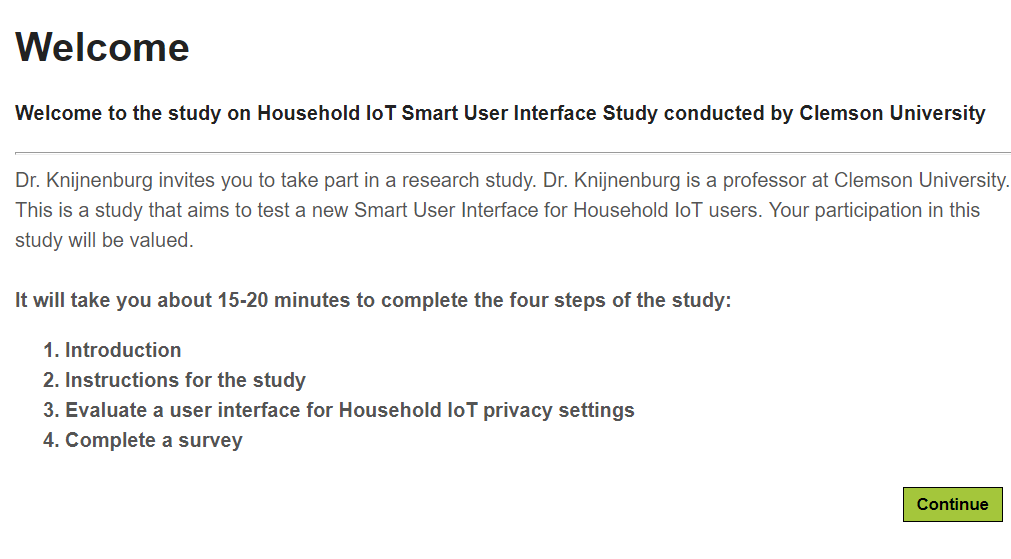
\includegraphics[width=0.48\textwidth]{figures/userstudy1.png}
	\caption{Experiment Landing Page}
	\label{fig:us1}
\end{figure}

\begin{figure}
	\centering
	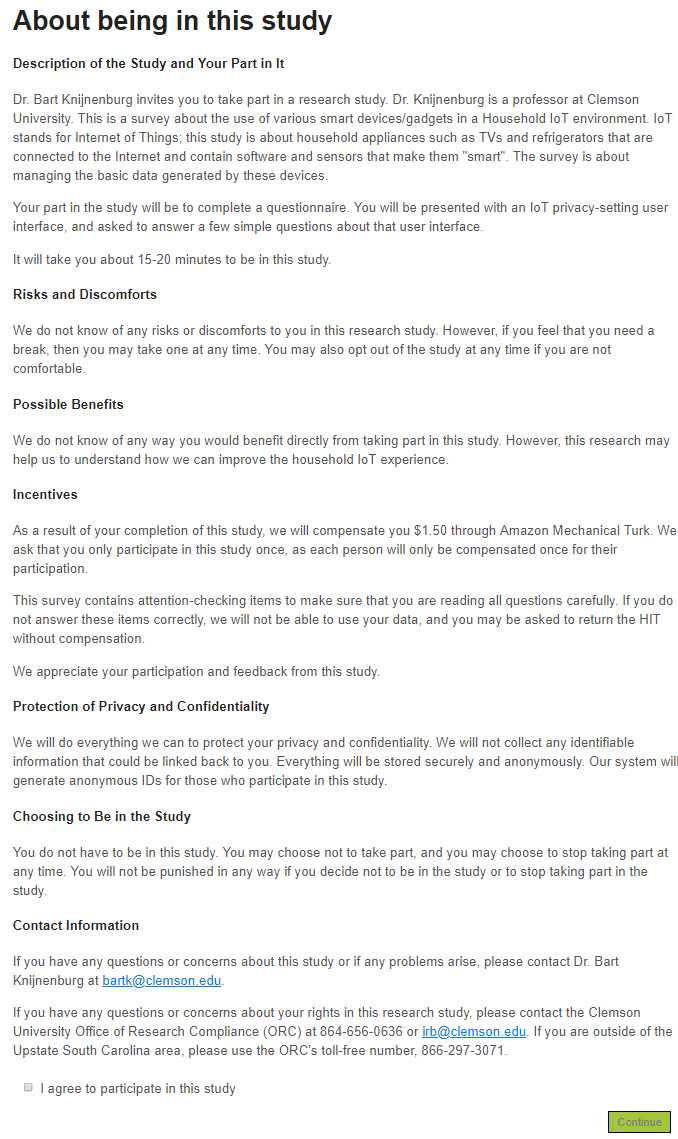
\includegraphics[width=0.48\textwidth]{figures/userstudy2.png}
	\caption{User Consent Form}
	\label{fig:us2}
\end{figure}

Then the participants will be introduced with the concept of the household IoT devices that appearing in this study, corresponding to the `Who' and `What' parameters of an IoT scenario. As shown in Figure~\ref{fig:us3}, the introduction contains both figures, text, and audio information. After the introduction, the participant will be given an example scenario to further understand the context of our study. Attention checks will also be given here to make sure the participants have paid attention to the explanations.
\begin{figure}
	\centering
	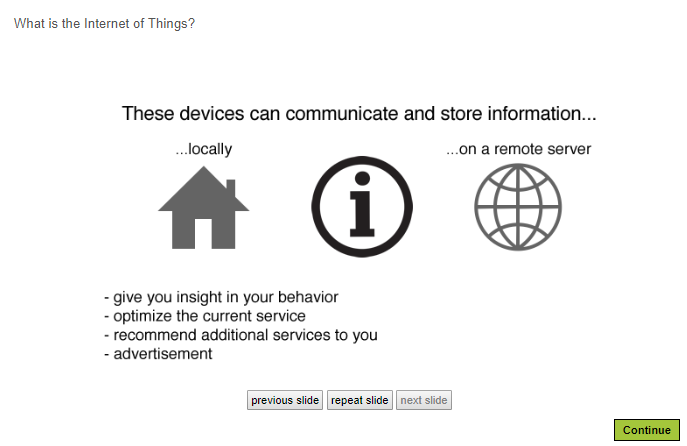
\includegraphics[width=0.48\textwidth]{figures/userstudy3.png}
	\caption{Introduction to Household IoT}
	\label{fig:us3}
\end{figure}

After above procedures, one out of the 8 user interfaces will be randomly chosen for each participants. Participants need to go through the whole interface to see if the preset privacy settings is suitable for them, and make necessary changes to accommodate their actual privacy demands. All these changes will be recorded to compared with the preset settings for further analysis purpose. A simple user interface condition with all settings turned off is shown in Figure~\ref{fig:ui1AllOff}.

\begin{figure}
	\centering
	\begin{subfigure}[t]{0.24\textwidth}
		\centering
		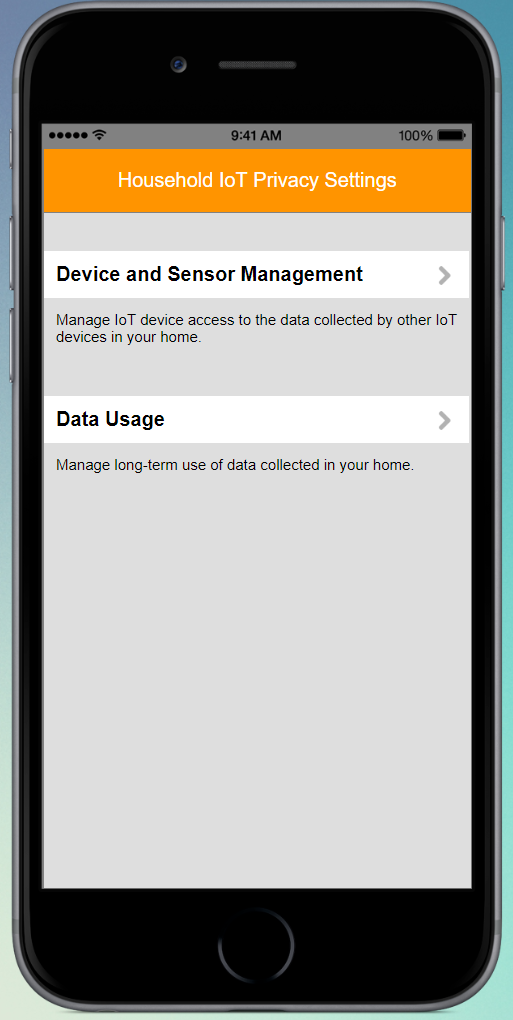
\includegraphics[height=2.8in]{figures/ui1allOff.png}
	\end{subfigure}%
	~
	\begin{subfigure}[t]{0.24\textwidth}
		\centering
		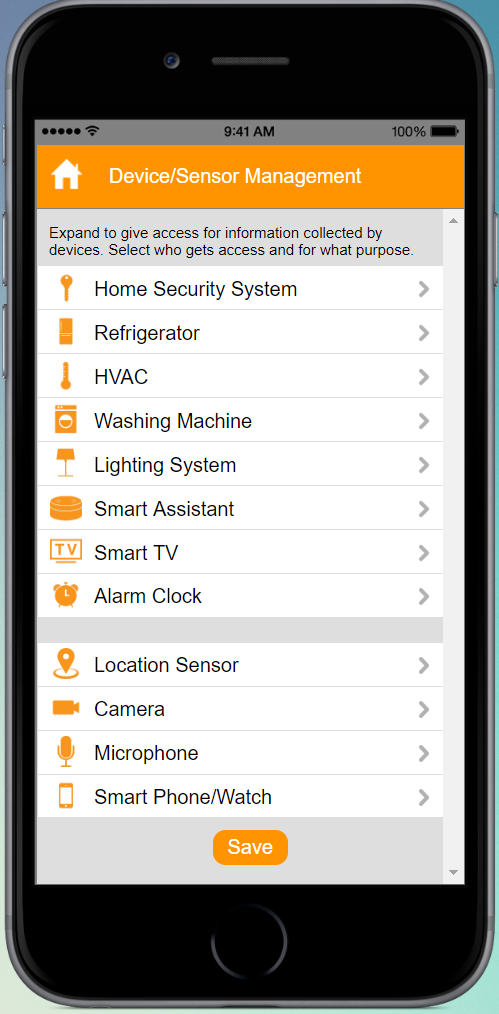
\includegraphics[height=2.8in]{figures/ui1allOff2.png}
	\end{subfigure}%
	~
	\begin{subfigure}[t]{0.24\textwidth}
		\centering
		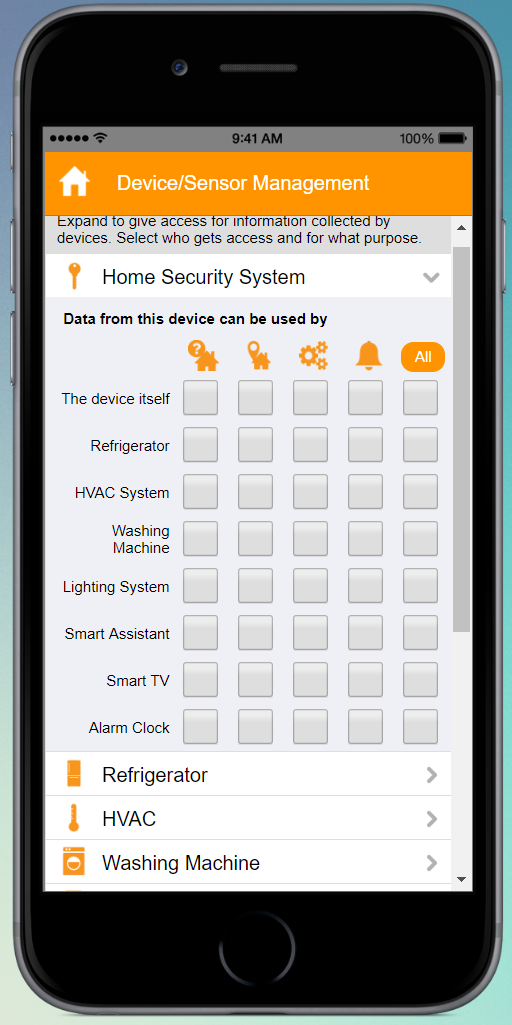
\includegraphics[height=2.8in]{figures/ui1allOff3.png}
	\end{subfigure}%
	~
	\begin{subfigure}[t]{0.24\textwidth}
		\centering
		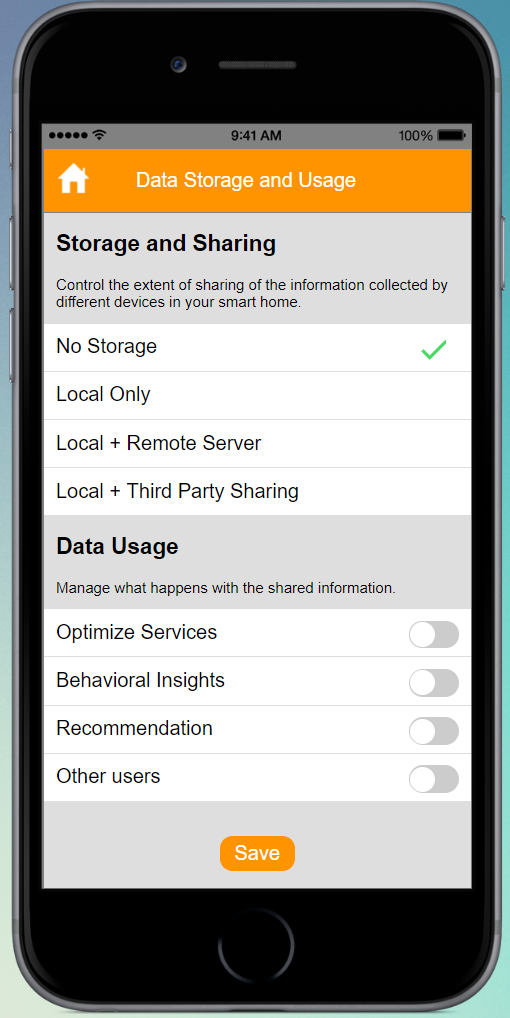
\includegraphics[height=2.8in]{figures/ui1allOff4.png}
	\end{subfigure}%
	\caption{Simple User-Interface condition with all settings turned off}
	\label{fig:ui1AllOff}
\end{figure}

Next, the participants will be give a survey containing questions about three different aspects: \textit{Subjective System Aspects} (Orange color), \textit{Personal Characteristics} (Blue color), and \textit{Situational Characteristics} (Green color), as shown in Figure~\ref{fig:uimodel}. All the items of the questionnaire are shown in Appendix.

\subsection{Measurements}
Two paper-based surveys will be constructed: 1) a pretest questionnaire consisting of three
parts (demographic, perceived sensitivity of the photo and willingness to share, privacy consciousness),and 2) a posttest questionnaire consisting of three parts (perceived sensitivity of the photo and willingness to share, usability, qualitative feedback).

\subsubsection{Pre-test survey}
The first part of the pretest survey elicits the following demographic data: gender, age,
ethnicity, employer, education, marital status, Internet usage, social media usage, and photo uploading
frequency. The second part of the pretest survey aims at assessing users' perceived privacy
of the sensitive photo and their willingness to share this photo without any privacy protection. All
the responses used 7-point Likert scale from 1 `Strongly disagree' to 7 `Strongly agree.' The two
questions are:
1) I feel my privacy can be compromised because the sensitive content can be learned from this
photo [10].
2)  I am willing to share this photo on my Facebook [52].
The third part consists of two questions on users' privacy consciousness (7-point Likert
scale) [139]:
3) Please tell us how important the following is to you: Being in control of what information is
collected about you.
4) Please tell us how important the following is to you: Being in control of who can get information
about you.

\subsubsection{Post-test survey}
The firrst part of the post-test survey is the same as the second part of the pre-test survey
which assesses users' perceived privacy of the photo and their willingness to share this photo with
the privacy enhancement. Next, the lite version of the Usability Metric for User Experience (UMUXLite)
is used to measure the system usability [124]. UMUX-Lite is a promising shorter alternative
to the commonly used System Usability Scale (SUS). It shows high internal reliability similar to the
SUS [124]. UMUX-Lite uses the 7-point Likert scale with the following two items:
This system's capabilities meet my requirements.
This system is easy to use.
At the end of the post-test survey, participants could provide their qualitative feedback on
our system.


\subsection{Procedure}
After signing a consent form, researchers introduce that the goal of this study is to investigate
the performance of a Facebook feature. In the control group, participants use their own Facebook
account. In two experimental groups, participants are provided with a Facebook account prototype
which mimics their own Facebook accounts (e.g., their Facebook data is shown in the prototype).
We first show them the sensitive photo that they share with us before the experiment. Note that
this photo is the one that they really want to share on Facebook despite some sensitive content.
Participants then answer the pre-test survey. Afterwards, they take different steps to post this photo
depending on which group they are in. Upon completion, participants then answer the post-test
survey. During the testing, we encourage them to think aloud and provide their suggestions and
confusions.

\subsection{Expected Results}

\begin{figure}
	\centering
	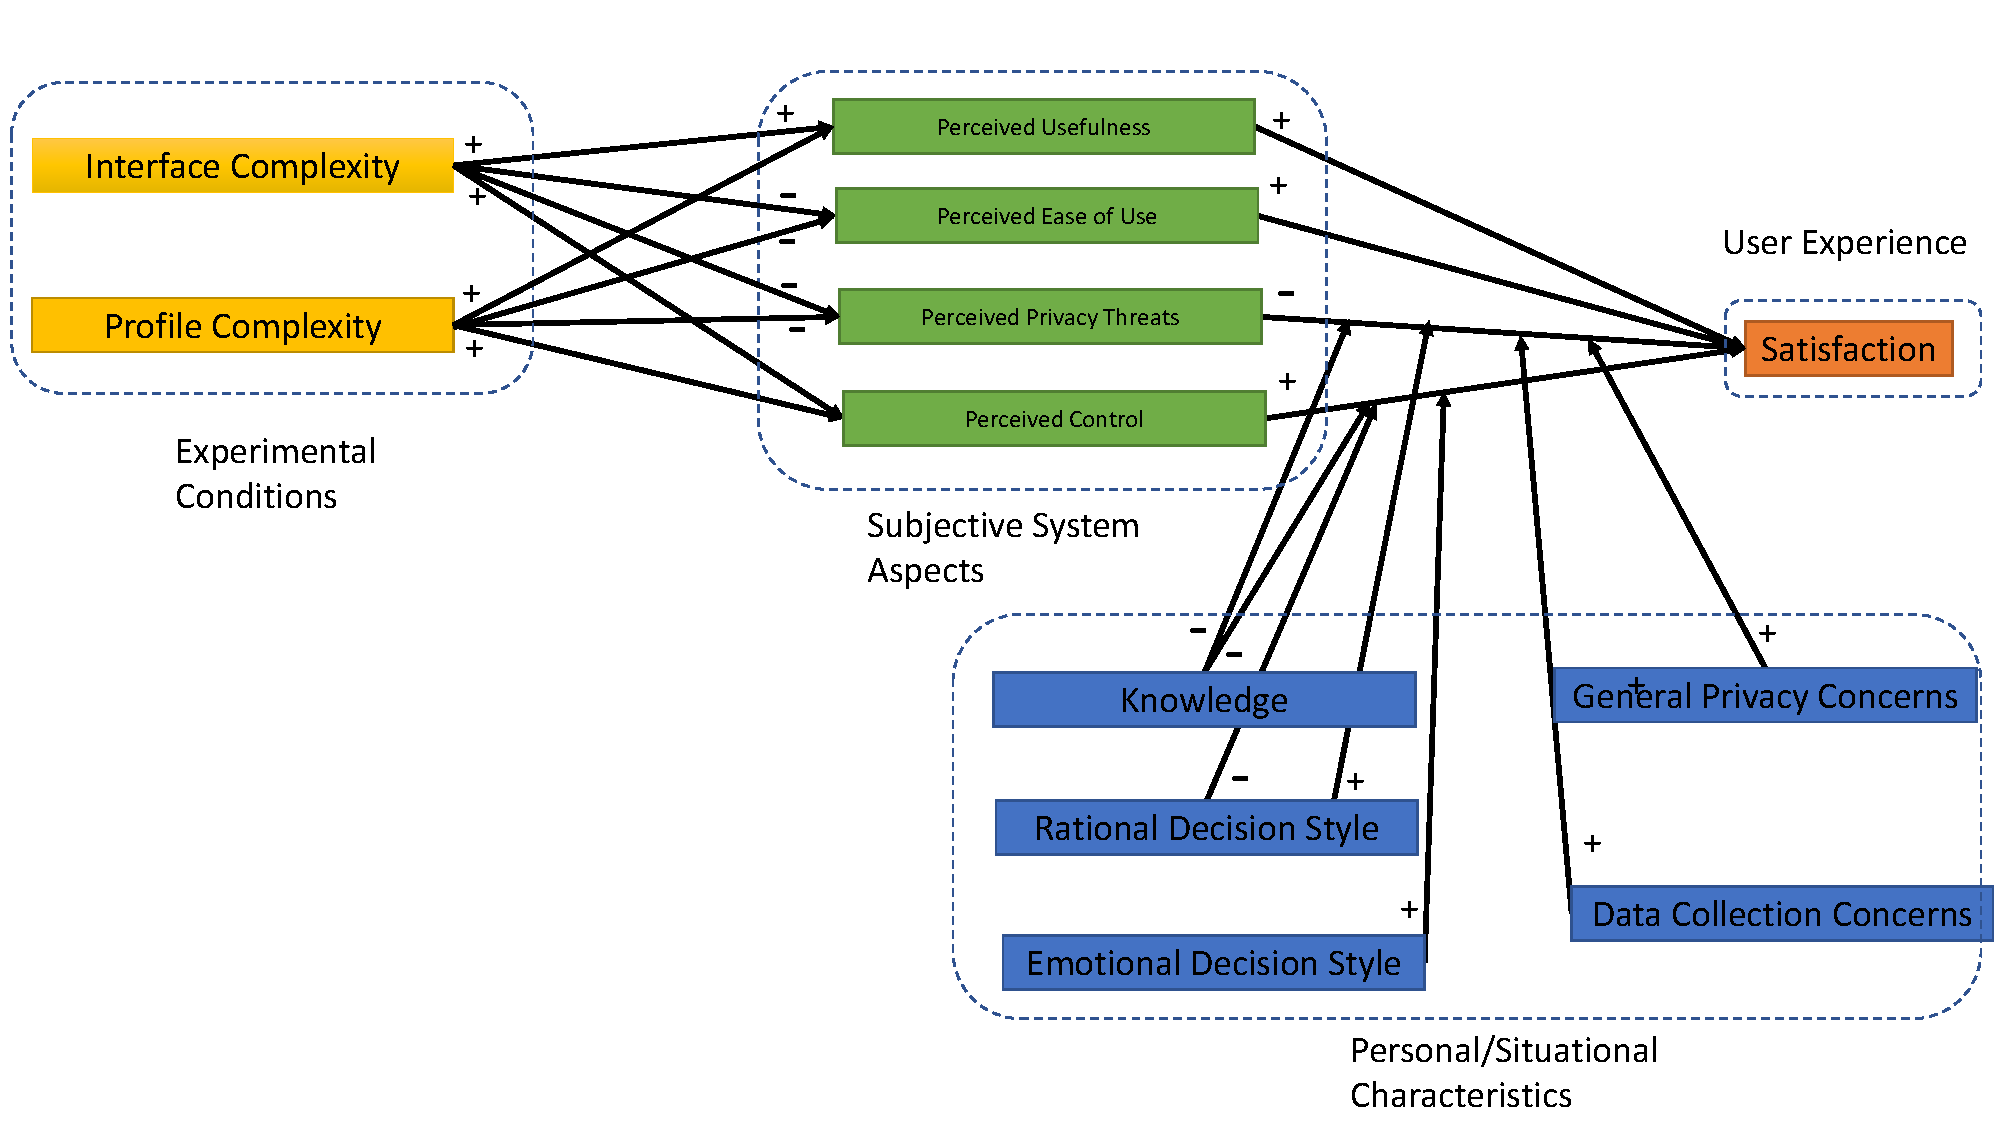
\includegraphics[width=0.9\textwidth]{figures/uimodel.pdf}
	\caption{Expected Structural Model for Proposed User Study}
	\label{fig:uimodel}
\end{figure}

As shown Figure~\ref{fig:uimodel}, we expect `General Privacy Concerns', `Data Collection Concerns', and 'Knowledge' all have a positive effect on the `Perceived Privacy Threats', which consequently has a negative effect on the `Trust' and `Satisfaction'. The mediation effect of `Trust' on `Satisfaction' will also be investigated. The effect of user's decision style is also interesting to us since different style of decision making may have effect on `Perceived Control' or `Perceived Privacy Threats', which will then affect user's `Trust' and `Satisfaction'. `Interface Complexity' is expected to have a positive effect on`Perceived Interface Complexity`, `Perceived Profile Setting Match', `Perceived Control', and `Perceived Ease of Use', which will have a positive effect on `Trust' and `Satisfaction'. `Profile Consevativeness' is expected to have a negative effect on `Perceived Privacy Threats' and a positive effect on `Perceived Control', which will then have a positive effect on both `Trust' and `Satisfaction'.

After the user study is finished, We will use statistics to analysis the effect of the independent variables on the subjective system aspects, and further mediation effect on the user experience. We also wonder how the personal characteristics ans situational characteristics affect the user experience. Finally, we will apply machine learning techniques to uncover deep insights of the results.